%%%%%%%%%%%%%%%%%%%%%%%%%%%%%%%%%%%%%%%%%%%%%%%%%%%%%%%%%%%%%%%%%%%%%%%%%%%%%%%%%%%%%%%%%%%%%%%%%%%%%%
%
%   Filename    : chapter_3.tex 
%
%   Description : This file will contain your Theoretical Framework.
%                 
%
%%%%%%%%%%%%%%%%%%%%%%%%%%%%%%%%%%%%%%%%%%%%%%%%%%%%%%%%%%%%%%%%%%%%%%%%%%%%%%%%%%%%%%%%%%%%%%%%%%%%%%

\chapter{Theoretical Framework}
This section discusses relevant theories and concepts to be used in the course of designing or developing the thesis.

\section{Speech Theory}

\subsection{Phonetics}
Phonetics focuses on the study of speech sounds, physiological production and their acoustic qualities. It is comprised of three branches. Articulatory Phonetics deals with the movement of the vocal organs that produces speech sounds. Acoustic Phonetics pertains to the acoustic properties of speech sounds; how the sound is being transmitted from the speaker to the listener. Lastly, Auditory Phonetics refers to the reception and perception of the listener \cite{britannica:2014:phoetics}.

\subsubsection{Articulatory Phonetics}
The traditional method of describing the physiological production of sound is through the vocal organs that produces them. The production of sound requires the use of the lungs, respiratory system, altogether with the vocal cords.

Speech sounds are separated into two major divisions, vowels and consonants. Vowels includes sounds that are produced without any major constrictions in the vocal tract. In the formation of consonants however, the airstream though the vocal tract is obsturated in a certain way \cite{britannica:2014:phoetics}.

\subsubsection{Acoustic Phonetics}
% Source: http://www.britannica.com/science/phonetics/Acoustic-phonetics

\begin{figure}[ht]
    \centering
    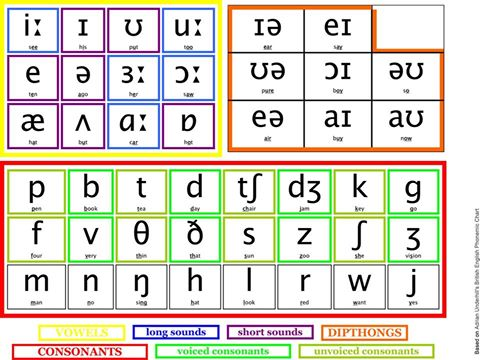
\includegraphics[totalheight=0.2\textheight]{diphthong-chart.jpg}
    \caption{Blue, J. (2013). }
    \cite{usingphonemes:img}
    \label{fig:diphthong-chart}
\end{figure}

Sounds that are produced by individuals differ from one another; varying in pitch, loudness, and quality. There are certain types of sounds that consists of periodic waves, one of which is the voiced sound. A voiced sound's pitch is determined in its fundamental frequency, or rate of repetition of the cycles of air pressure. The loudness of the voiced sound is dependent on the amplitude of the pulses of air pressure produced by the vibrating vocal cords. Pulses of air with a larger amplitude have a larger increase in air pressure. The smaller vibrations help determine the quality of a sound. Moreover, these smaller variations in air pressure correspond to the overtones that occur above the fundamental frequency \cite{britannica:2014:acoustic-phoetics}. 

\subsection{Phonemes}
Phonemes are singular units of sound. These set of units are comprised of all the vowels and consonants in the English alphabet, arranged and grouped according to their characteristics \cite{wikipedia:2014:phoneme}. Phonemes are categorized into two classes: Vowels, Consonants. Vowels are further divided into two classes, monothongs, which is subdivided into long ang short vowel sounds, and diphthongs. Consonants are also split into two categories, the unvoiced consonants and the voiced consonants \cite{jadeblue:2013:phonemic-chart}. 

\subsubsection{Diphthongs}
In linguistics, diphthongs, also known as gliding vowels, are a combination of two different vowel sounds. Compared to vowel sounds, diphthongs occur when a vowel sound is produced and the tongue moves during the pronunciation of the aforementioned vowel \cite{britannica:2015:diphthongs}.

\section{Feedback Mechanisms}

Feedback is considered either a positive or a negative one. A positive feedback is called "positive reinforcement" while a negative feedback is called "punishment" \cite{brookhart:2008:gef}. These feedback theoretically affect learning; however, not all feedback are effective \cite{brookhart:2008:gef}.


\begin{comment}
\begin{table}[!htbp]   %t means place on top, replace with b if you want to place at the bottom
\centering
\caption{Table of Feedback Strategies} \vspace{0em}
\begin{tabular}{|p{1in}|p{1.5in}|p{2in}|}
 \hline
\centering
Feedback Strategies May Vary In... & In These Ways... & Recommendations for Good Feedback \\ \hline
    Timing
    & \begin{itemize}
        \item When given
        \item How often
      \end{itemize}
    & \begin{itemize}
        \item Provide immediate feedback for knowledge of facts (right/wrong).
        \item Delay feedback for more comprehensive reviews of student thinking and processing.
        \item Never delay feedback when it would make a difference to students.
        \item Provide feedback as often as is practical, for all major assignments.
        \end{itemize}
        \\ \hline
    Amount
    & \begin{itemize}
        \item How many points made
        \item How much about each point
        \end{itemize}
    & \begin{itemize}
        \item Prioritize - pick the most important points.
        \item Choose points that relate to major learning goals.
        \item Consider the student's developmental level.
        \end{itemize}
        \\ \hline
    Mode
    & \begin{itemize}
        \item Oral
        \item Written
        \item Visual Demonstration
        \end{itemize}
    & \begin{itemize}
        \item Select the best mode for the message Would a comment in passing the student's desk suffice? Is a conference needed?
        \item Interactive feedback (talking with the student) is best when possible.
        \item Give written feedback on written work or on assignment cover sheets.
        \item Use demonstration if "how to do something" is an issue or if the student needs example.
        \end{itemize}
        \\ \hline
    Audience
    & \begin{itemize}
        \item Individual
        \item Group/class
        \end{itemize}
    & \begin{itemize}
        \item Individual feedback says, "The teacher values my learning."
        \item Group/class feedback works if most of the class missed the same concept on an assignment, which presents an opportunity for reteaching.
        \end{itemize}
        \\ \hline
\end{tabular}
\label{tab:feedback-strategy-table}
\end{table}
\end{comment}

\begin{figure}[ht]
    \centering
    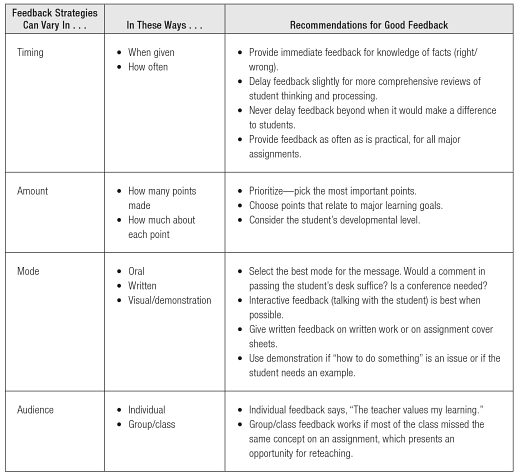
\includegraphics{feedback-strategy-table.PNG}
    \caption{Feedback Strategies Table (Brookhart, 2008)}
    \label{fig:feedback-strategy-table}
\end{figure}

Certain strategies are used to give feedback in different ways. These strategies may vary in Timing, Amount, Mode, and Audience while the feedback content may vary in focus, comparison, valence and other variations \cite{brookhart:2008:gef}. Timing strategy refers to when a feedback should be given and how often it should be given. A feedback may be given immediately if the output needed is factual or may be delayed if it requires more analysis. Generally, the feedback should be given as often as needed. Amount of feedback to be given to the students depending on how many important points are needed, for example, if a student is learning speech, certain points to consider are the accent and the grammar of the student. The mode of showing the feedback varies in oral, written or visual demonstration. Interactive feedback are considered best, which means it relates the performance of the student to actual task. Audience refers to how many students are receiving feedback. It may be individual or in a group or class. Individual feedback makes the student realize that the teacher is focused on their learning while group or class feedback is best used when most of the class have the same misunderstanding which may lead to reteaching.

The use of different feedback strategies depend on which part a student should improve on or when it should be given as shown in \figref{fig:feedback-strategy-table}. 

\subsection{Mode Strategy}
Feedback in a form of mode may be shown in oral, written or other visual demonstration. One visual demonstration may be used is showing it in a "how it should be done" form. It may be demonstrated by a person or by a video playback.

% FEEDBACK, MORE THAN JUST YES AND NO
% How are people visualising it?
\subsection{Traditional Methods}
% What are traditional ways & methods?

\begin{comment}
Various ways to teach speech to the deaf were invented and developed since it was pioneered in the 16th century \cite{markides:1983:sohic}. It started with Pedro Ponce de Leon, a Benedictan monk in Spain, who first started teaching speech to the Deaf when he met two deaf boys and was put under the care of the monastery \cite{markides:1983:sohic}.
\end{comment}

Currently, traditional ways of teaching speech requires the aid of a speech therapist and not only teach children with hearing-impairment how to speak but also children with Down syndrome, motor speech disorders, developmental delays and other speech disorders. Various speech therapies may be used depending on the disorder the child has. A speech therapy's purpose is to systematize the mechanics of speech with the use of language and it is often included in autism behavioral intensive programs \cite{autispks:2015:slmi}. Developmental verbal dyspraxia, a disorder that makes a child unable to speak sounds and words well, may also be managed by a different type of speech-language therapy. Aphasia is another condition wherein a person is having difficulties in speaking due to brain damage \cite{damasio:1992:aphasia} which happens after a person had experienced stroke. Speech therapy helps them by giving drills to improve specific language skills, group therapy to improve conversational skills, and augmenting their communication skills through gestures and writing \cite{hayes:2013:tost}.

Other conditions and disorders that may be treated by speech therapy, as listed by Hayes \citeyear{hayes:2013:tost}, are stuttering, swallowing difficulties, and children who are late talkers.

\subsection{Speech Training for the Hearing-Impaired}
Speech Training systems that were previously implemented focused on the visual stimuli of the Deaf students in order to learn speech. However, the method of providing feedback differed from one software to another, only dealing with a certain topic for the student to learn.

The software SpeechViewer III, developed by IBM, was created to develop the vocal skills of the hearing-impaired \cite{speechville:2014:slp}. By transforming a user's speech to a graphically represented model, the students are motivated to continue developing their voicing, pitch, loudness, phoneme accuracy and speech timing \cite{kennedy:1998:spv}.

Similarly, Speech Therapy 5, offers the same capabilities of SpeechViewer 3. However, it has expanded to over 70 types of games, allowing the student to futher practice speech. Speech Therapy 5 has also allowed the student's supervisors to provide additional feedback as the program provides graphical display and statistical data of the students's performance \cite{drspeech:1998:st5}.

Video Voice, another speech training system that has been providing assitance to hearing-impaired indivuals for more than 35 years, has expanded its faculties by accomodating almost any type of speech work \cite{videovoice:2015:description}. Video Voice also displays its feedback by means of a gamified graphical representation of an individual's speech \cite{videovoice:2015:speechtherapyapplications}. In addition, Video Voice renders formants for every individual, displaying their performances on various models in order for their therapists to select the appropriate therapy targets \cite{videovoice:2015:formantdisplays}.

\subsection{Speech Training for Children}

Numerous Speech Training systems and methods, in both computerized and traditional, have been constructed to benefit other individuals with different disablities or impairments. 

A system has been developed in order to cater the needs of language-learning impaired children, who are having difficulty in learning their native language. Through the use of an algorithm that renders the volume of rapidly change elements in speech, to make them salient, they futher improved on their performance \cite{jstor:1996:lli}. Schizophrenic Children on the other hand were taught through series of verbal discrimination, being rewarded as they are able to replicate the adult's speech \cite{science:1966:schizo}.

Through the use of the picture exchange communication system (PECS), an augmented and alternative communication, allows children with autism to learn communication by means of exchanging pictures for items or activites they are interested in \cite{wiley:2002:pictureexchange}. 

Children with spoken language impairment (SLI) often shows signs of early reading delay. Such impairment demonstrated expressive phonological difficulties, more so, had retarded development of their semantic and syntactic skills \cite{lshss:2000:sli}. Through the introduction of the integrated phonological awareness intervention to these preschool children, it has assisted them in developing their speech. with spoken language impairment, students undergo series of speech production, phonological awareness and letter-sound knowledge \cite{gillonmcneill:2007:sli}.

Bungalow Software, is a speech and language recovery system for patients recuperating from after stroke traumatisation, aphasia, or brain injury. This software was designed to work a way such that a speech pathologist is providing series of drill therapies to the patient. Series of questions is asked to the patient, where they will have to try answering each question until they provide the correct answer. By instant grading and giving hints to the patients, they are motivated and are able to learn faster \cite{bungalow:2012:speechtherapy}.

\subsection{Accent Traning}
% Call Center Agent Accent Training
Accent is simply defined as a distinctive way of speaking speech sounds and it is associated within a certain group or nation \cite{adams:2009:sgsa}. Some people attempt to change their accents to improve within the field of their work \cite{ravin:2004:lyad}. Currently, one may get accent trainings through online courses or with the aid of self-help books such as Jennifer Adams and Johanna Chapman's \citeyear{adams:2009:sgsa} and Judy Ravin's \citeyear{ravin:2004:lyad} books.

Generally, a person may change or imrpove their accent by surrounding themselves with people having the accents they want to acquire and listen to them closely \cite{omniglot:2015:ttiya}. Another is by attempting to speak in that target accent which may be practiced by reading sentences aloud or listening to a practice module consistently \cite{omniglot:2015:ttiya}. Courses and books train students to a more focused scope in the accent. It usually starts with speaking certain vowels and consonants using the target accents and linking the vowels and consonants together and, finally, applying it to conversations and informal speech \cite{ravin:2004:lyad}.

% --------- CS FRAMEWORK ---------

\section{Self-Organizing Maps (SOMs)}
Self-organizing map (SOM) is an artificial neural network that discovers patterns in the input data and can learn even without supervision \cite{kohonen:1988:pho}. It transforms multi-dimensional inputs into a two-dimensional mapping and each output in the map is given a weight \cite{chandar:2013:srs}. SOMs may be used to detect or map a vowel sound based on a user's voice input. 

The map consists of grid of squares called "nodes". Each node is equivalent to a category (or a combination of the different dimensions of data depending on the intensity of each dimension). It is also ensured that topology is reserved which means that a node has a great relation between other neighboring nodes \cite{li:2008:som}.

At the start, the neurons are given random weight values. This is called the initialization phase. The next step of the process is determining which neuron is closest to the input via its given weight value. "The weights of the winning neuron and neurons close to it in the SOM lattice are adjusted towards the input vector" \cite{chandar:2013:srs}. This is called the competition phase \cite{agustin:2014:SOM}. Lastly, the weight of the winning neurons and its neighbors are adjusted in relation to the input pattern in this third phase called adaptation phase, hence, the SOM is created.

% The input of the her thesis is not sound, but processed sound or audio which is converted to CSV.
\begin{comment}
For example, considering Natalie Agustin's \citeyear{agustin:2014:SOM} thesis, the input of the system would be sound or audio, specifically vowel sounds from the user's voice. The 5 basic vowel sounds ('a', 'e', 'i', 'o', 'u') are considered to their own nodes (category) and everything else in between (i.e. combination of 'a' and 'e' sound or longer 'oo' sound) will have their own nodes as well. The basic vowels are identified as the different dimensions, meaning we have 5-dimensional data. Once the system read an input, it will weigh in each dimension to the input and will be mapped accordingly to a node.
\end{comment}

\section{Mel-Frequency Cepstral Coefficients (MFCC)}
% Still incomplete. Add info about the other steps but not too detailed.
The Mel-Frequency Cepstral Coefficients (MFCC) is common for translating speech sound into coefficients and has succeeded because of representing the speech amplitude spectrum in a compact form \cite{logan:2000:mel}. Out of all existing feature extraction models, MFCC is the most popular and has become the standard in speech recognition systems \cite{Sahidullah2012543}. MFCC is a good feature extraction model as it discards unneeded data (background noise, emotion, etc).

This feature extraction model generally consists of five steps: Windowing, Taking the Discrete Fourier Transform (DFT), Applying the Mel Filterbank, Taking the Log of All Filterbank Energies and Taking the Discrete Cosine Transform.

The windowing step divides the audio into several windows and is described more in detail in the following subsection. The DFT extracts which frequencies are present from each frame. However, the output of the DFT still contains unneeded information for speech recognition which is why each frame goes through a filterbank which outputs how much energy exists in each frequency band. Taking the log from each filter from the previous step allows usage of ceptral mean subtraction, a channel normalisation technique. The final step computes the DCT of the log filterbank energies which outputs the Mel-Frequency Cepstral Coefficients.

\subsection{Windowing}
In this step, the audio is divided into several windows, each having an interval of usually 20 milliseconds (also called the frame size). Each window is statistically stationary, making feature extraction less complex as the sounds of each window are static.

The problem with speech is that it is not stationary, sound and pitch change throughout the speech, thus may face issues when performing the latter parts of the MFCC model. The windowing step is designed to make the speech (or parts of the speech) stationary by dividing it into windows. There are configurations before performing windowing. First, the frame size is to be determined. The frame size defines how long (in milliseconds) a frame is. Usually, 20 milliseconds is set as the frame size \cite{han:mfcc-extraction:2006}. Second, the frame shift is also to be determined. The frame shift is the offset between windows \cite{agustin:2014:SOM} and is usually set to 10 milliseconds \cite{han:mfcc-extraction:2006}.

\begin{figure}[h]
    \centering
    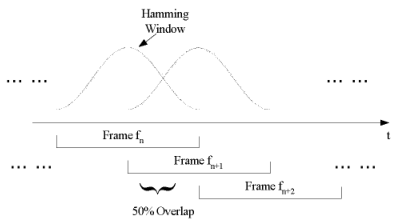
\includegraphics{hamming-window.PNG}
    \caption{Frame blocking in the MFCC extraction algorithm (Han et al., 2006)}
    \label{fig:hamming-window}
\end{figure}

One issue present when cutting audio into several windows is that these windows are snipped instantly, causing high frequency noises at each frame's start point and end point due to sudden change \cite{han:mfcc-extraction:2006}. The Hamming window is used to reduce or stabilize a frame's frequency noise. As shown in \figref{fig:hamming-window}, the maximum height of a frame is similar to the other frames.

\section{Agustin's Research}
Natalie Agustin's research uses Self-Organizing Maps and regression models in order to display Visual Articulatory Feedback (VAF). Agustin's VAF displays how articulations---speech organs which produce sound---are formed when pronouncing a vowel. Agustin's software prototype takes audio (vowel pronunciation) as input and outputs the VAF. Models created in her research are from the MOCHA-TIMIT dataset, which were created by The University of Edinburgh's Centre for Speech Technology Research. The MOCHA-TIMIT dataset provides a phonetically balanced dataset for training an automatic speech recognition system. The VAF is shown in side view, displaying vocal tracts on a shape of a face drawn on a plotted Cartesian map.

Agustin's purpose for the research was to create a VAF system for speech learning of people with hearing impairment. Agustin developed a prototype which visually displays the articulations that need to be formed in order to speak the targeted sound.

Agustin has provided the researchers of this paper with her method of training data with the use of EMA files from the MOCHA-TIMIT dataset. This will allow the researchers to change the dataset, that instead of vowels, a fixed set of phonemes will be used. Also, the SOM algorithm by Agustin will be used by the researchers as well which will be needed in the feedback system in determining how far or how near the trainee is from the targeted pronunciation.